\documentclass{sigchi}

% Use this command to override the default ACM copyright statement (e.g. for preprints). 
% Consult the conference website for the camera-ready copyright statement.
\toappear{
Permission to make digital or hard copies of all or part of this
work for personal or classroom use is granted without fee provided that 
copies are not made or distributed for profit or commercial advantage and
that copies bear this notice and the full citation on the first page. To
copy otherwise, or republish, to post on servers or to redistribute to 
lists, requires prior specific permission and/or a fee.\\
{\confname{CSCW'15}},	  March 14-18, 2015 in Vancouver, Canada\\
}

\toappear{\scriptsize Permission to make digital or hard copies of all or part of this work for personal or classroom use is granted without fee provided that copies are not made or distributed for profit or commercial advantage and that copies bear this notice and the full citation on the first page. Copyrights for components of this work owned by others than ACM must be honored. Abstracting with credit is permitted. To copy otherwise, or republish, to post on servers or to redistribute to lists, requires prior specific permission and/or a fee. Request permissions from permissions@acm.org. \\
{\emph{CSCW 2015}}, March 14--18, 2015, Vancouver, BC, Canada. \\
Copyright is held by the owner/author(s). Publication rights licensed to ACM. \\
ACM 978-1-4503-2922-4/15/03\ ...\$15.00.\\
http://dx.doi.org/10.1145/2675133.2675286}
\clubpenalty=10000
\widowpenalty = 10000

% Arabic page numbers for submission. 
% Remove this line to eliminate page numbers for the camera ready copy
%\pagenumbering{arabic}


% Load basic packages
\usepackage{balance}  % to better equalize the last page
\usepackage{graphics} % for EPS, load graphicx instead
\usepackage{times}    % comment if you want LaTeX's default font
\usepackage{url}      % llt: nicely formatted URLs

% llt: Define a global style for URLs, rather that the default one
\makeatletter
\def\url@leostyle{%
  \@ifundefined{selectfont}{\def\UrlFont{\sf}}{\def\UrlFont{\small\bf\ttfamily}}}
\makeatother
\urlstyle{leo}


% To make various LaTeX processors do the right thing with page size.
\def\pprw{8.5in}
\def\pprh{11in}
\special{papersize=\pprw,\pprh}
\setlength{\paperwidth}{\pprw}
\setlength{\paperheight}{\pprh}
\setlength{\pdfpagewidth}{\pprw}
\setlength{\pdfpageheight}{\pprh}

% Make sure hyperref comes last of your loaded packages, 
% to give it a fighting chance of not being over-written, 
% since its job is to redefine many LaTeX commands.
\usepackage[pdftex]{hyperref}
\hypersetup{
pdftitle={SIGCHI Conference Proceedings Format},
pdfauthor={LaTeX},
pdfkeywords={SIGCHI, proceedings, archival format},
bookmarksnumbered,
pdfstartview={FitH},
colorlinks,
citecolor=black,
filecolor=black,
linkcolor=black,
urlcolor=black,
breaklinks=true,
}

% create a shortcut to typeset table headings
\newcommand\tabhead[1]{\small\textbf{#1}}


% End of preamble. Here it comes the document.
\begin{document}

\title{The Virtuous Circle of Wikipedia\\ \vspace{0.3cm} {Recursive Measures of Collaboration Structures}\\ \vspace{0.3cm}}

%\numberofauthors{1}
%\author{[anonymized author names and affiliations]}


\numberofauthors{3}
\author{
\alignauthor
Maximilian Klein\\
       \affaddr{OCLC Research}\\
       \affaddr{777 Mariners Island Blvd}\\
       \affaddr{San Mateo, CA, 94404}\\
       \email{kleinm@oclc.org}
% 2nd. author
\alignauthor
Thomas Maillart\\
       \affaddr{School of Information}\\
       \affaddr{ University of California, Berkeley, 102 South Hall}\\
       \affaddr{Berkeley, CA 94720}\\
       \email{maillart\\@ischool.berkeley.edu}
% 3rd. author
\alignauthor
John Chuang\\
       \affaddr{School of Information}\\
       \affaddr{ University of California, Berkeley, 102 South Hall}\\
       \affaddr{Berkeley, CA 94720}\\
       \email{chuang\\@ischool.berkeley.edu}
}

% Teaser figure can go here
%\teaser{
%  \centering
%  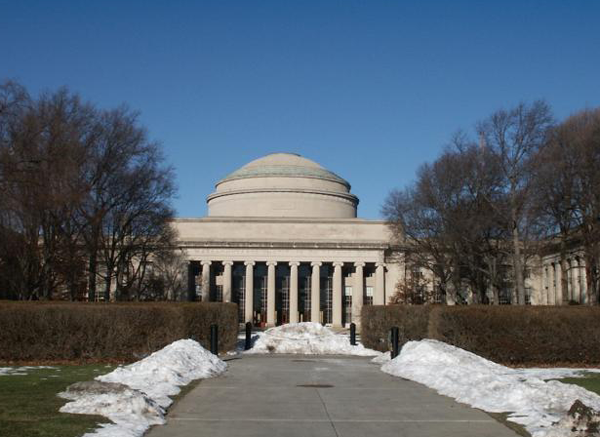
\includegraphics{Figure1}
%  \caption{Teaser Image}
%  \label{fig:teaser}
%}

\maketitle

\begin{abstract}
In open collaboration, knowledge is created and iteratively improved by a multitude of editors who freely choose what should be their contributions. The quality of knowledge artifacts (e.g. article, source code file) is deeply tied to their individual expertise, and to their ability to collaborate well. Conversely, the expertise of contributors is a function of artifacts contributed to. Building upon a large stream of literature on the measurement of article quality and contributor expertise, we propose a recursive algorithm to measure how editor expertise influences the quality of articles, and how contributions to articles influence editor expertise. This {\it bi-partite network random walker} metric reveals the specific structure of cooperation and how the quality of articles is achieved through coordination. We show that while the wisdom of crowds is well pulled in some categories, more editors per article can also create disvalue.
\end{abstract}


%\textcolor{red}{The following section is mandatory for accepted papers, but not needed for submissions for the June 1 deadline.}
\category{H.5.3}{[Information Systems]: Group and Organization Interfaces}{computer-supported collaborative work}

\keywords{open collaboration; bi-partite networks; performance; coordination}
%See: \url{http://www.acm.org/about/class/1998/}
%for more information and the full list of ACM classifiers
%and descriptors. 

%\textcolor{red}{The following section can be included for accepted papers, but is not needed for submissions for the June 1 deadline.}

%\terms{
%	Human Factors; Design; Measurement. 
%	If you choose more than one ACM General Term, 
%	separate the terms with a semi-colon.
%}

%See list of the limited ACM 16 terms in the
%instructions and additional information:
%\url{http://www.sheridanprinting.com/sigchi/generalterms.htm}.
%\textcolor{red}{Optional section to be included in your final version.}

\section{Introduction}
In online open collaboration knowledge, artifacts such as open source code, Wikipedia articles, and 3D-printing designs, are usually produced and improved collectively by a multitude of contributors. Some people devote numerous hours of labor improving existing content and adding new features, while most contributors only make minor changes. Yet, in addition to the power of the few, a mass of small changes can make the difference as a form of emergent collective intelligence \cite{kittur2007power}.  As the Internet has become pervasive in modern societies, open collaboration has permeated to a broad variety of social contexts and industries \cite{benkler2011leviathan}. 

Despite {\it bottom-up} self-organization, participants in open collaboration can collectively achieve  the production of high quality and reliable knowledge, as demonstrated for instance in Wikipedia \cite{giles2005internet}. This form of labor organization is called peer-production and it usually heavily relies on Internet communication systems. Peer-production is based on {\it task self-selection} and {\it peer-review} \cite{benkler2002}: participants decide to contribute according to their skills, and in turn, skills are improved as they contribute more, and so on, following a virtuous circle.

Because open collaboration enjoys horizontal organization, the dynamics of contributions are contingent to the heterogenous motivations and incentives of participants \cite{vonKrogh2012}, and some knowledge artifacts enjoy various attention from the community, with time localized bursts for hot topics \cite{keegan2013hotoff}. These  highly non-linear, transient and intrinsically unpredictable bursts of iterative improvements are the hallmark of successfully organized communities \cite{vonkrogh2014designing}. They can be rationalized by critical cascades of both individual contributions and interactive community-based iterative improvements \cite{sornette2014howmuch}. {\it Individual} versus {\it interaction-based} mechanisms are hard to disentangle, and therefore, understanding the structure of collaboration remains a difficult challenge. For larger groups concentrating on precise problems (e.g., in open collaboration), interactions typically magnify coordination problems \cite{halfaker2013}. %Moreover, open collaboration projects unfold over large time scales of several years, sometime decades, and the lurking and learning-by-doing components play a crucial role in the engagement of contributors \cite{vonkrogh2003}. 

To understand the origins of cooperation structures and quality in open collaboration, we posit that the value of each knowledge artifact (e.g., source code file, article) is deeply tied to the expertise and the number of its contributors, who can witness potential mistakes or outdated information. Conversely, the expertise of contributors is a function of artifacts contributed to, and so on, recursively.

To measure how artifacts benefit from a larger number of editors with a given expertise, and how editors benefit from having contributed to more artifacts of some quality, we propose a {\it bi-partite network random walker} algorithm, which is a two node type extension of the recursive {\it pageRank} algorithm \cite{page1999pagerank,kleinberg1999}. We calibrate the algorithm on $12$ Wikipedia categories of articles, and we show, at the level of each category, how articles do (or do not) benefit from the intervention of more editors and their expertise.

The rest of this paper is organized as follows. We first expose the reader to the large literature on Wikipedia, measuring article quality, editor expertise and their mutual interplay. We then introduce the intuition behind the {\it bi-partite network random walker} algorithm, as well as its implementation for the present study. Data employed and the results are then presented and discussed. We finally conclude with limitations and future research directions.

\section{Related Work}
The structure and dynamics of individual and collective contributions have long since been recognized by researchers as primary factors for the achievement of high quality content, starting with scientific publications \cite{newman2001} and open collaboration projects \cite{bryant2005}. In the meantime, some of these open collaboration projects have tremendously increased their size and the number of their contributors, making it hard to assess the value of each knowledge artifact, even by intensive peer-review. The Wikipedia community, as well as researchers, have tried to find ways to determine article quality and editor expertise in a systematic way. These approaches have systematically faced criticism. Many quality article metrics have been proposed from methods based on word count \cite{blumenstock2008sizematters}, revision history \cite{hu2007articlequality},  general structure of articles \cite{wang2013tell}, patterns of changes between article versions \cite{woehner2009}, and combinations of type and volume of edits and editor expertise \cite{kane2011}. Editor expertise has also been investigated by considering  total number of words written, number of edits made, longevity of edits \cite{adler2008measuringauthor}, time spent in edit sessions \cite{geiger2013}, and number of {\it barnstars} collected \cite{Kriplean2008}. Other editor features that have received the attention of researchers include creative editing \cite{iba2010}, how power editors differ from normal editors \cite{panciera2009}, and the influence of the type of contributors on the quality of articles \cite{stein2007}.

The effort to measure article quality and editor expertise has extended to predicting the quality of contributions \cite{druck2008learning,zeng2006computingtrust}, developing reputation systems for editors \cite{adler2007contentdriven}, and identifying editor candidates for promotion \cite{burke2008taking}.

%\textcolor{red}{I think we can delete this paragraph, its off topic.}
%In contrast, the difficulty to assess the quality of artifacts and the expertise of editors differs with the ease to make the same evaluation with software code which can be compiled and tested. In a Matlab experiment for solving NP-hard problems, it was found that work shared as a public good helps individuals quickly reuse existing results, and thus, find better algorithms \cite{gulley2010}. Source code submissions by individuals programmers were tested and benchmarked for their capacity to solve the assigned problem quickly, by executing the compiled code on a computer. Unfortunately, for the time being, this approach is exclusively feasible for machine executable knowledge (i.e. software code) and in highly controlled environments.

We believe that the general skepticism about these metrics and reputation systems is grounded in their inability to capture and make sense of coordination between contributors. Coordination, defined as an on-going process that produces other measurable outcomes, is in general hard to understand in societies \cite{ostrom1990}. CSCW researchers have been specifically concerned with coordination viewed as a feature of a community, i.e., the effect of more peers on output quality. While collaboration and additional reviews by peers are generally perceived as positive, depending on the type of tasks and their required coordination, performance can also be undermined by inadequate coordination processes \cite{kittur2009coordination}. On the contrary, the effects of diversity on group productivity seem to increase group productivity \cite{chen2010}. It was also found that editors cluster by interest, with higher coordinated efforts in densely populated clusters \cite{jesus2009}. In particular, Wikipedia has been a heavily explored {\it field} for social scientists, starting with concerns on the effects of peer-review and whether single or repeated contributions by editors would help improve the quality of articles \cite{hu2007articlequality,wilkinson2007}. 

As an hybrid example, the specific problem of coordination in {\it featured} Wikipedia articles, which are heavily contributed over short time periods, has raised concerns on implicit versus explicit coordination processes and the limited positive quality it can bring when editors are too numerous \cite{kittur2008}.
 
The connection between article quality and editor expertise is present in nearly all literature aiming to understand the effects of the coordination process on the value of Wikipedia articles. The typical structure of networks with edges that connect uniquely two kinds of nodes is called {\it bi-partite} \cite{newman2001}. The analysis of patterns in Wikipedia bi-partite networks, with editors being one node type and articles the other, confirmed the existence of overlapping cliques of densely connected articles and editors  \cite{jesus2009}. A more detailed analysis of medical and health-related articles on Wikipedia, showed that the position of articles in the bi-partite network of articles and editors significantly influenced its quality \cite{kane2009}. 

Recent developments in the science of bi-partite networks has shown the feasibility to rank entities of each type through a recursive algorithm called  {\it method of reflections}.This method has been tested on the bi-partite network of countries exporting products \cite{hidalgo2007,hidalgo2009}. The method of reflections has been improved and complemented in more recent work, mainly to improve its robustness \cite{tacchella2012new, cristelli2012competitors, tacchella2013economic, cristelli2013measuring}. Caldarelli et al. \cite{caldarelli2012network} have proposed an alternative method, based on biased stochastic Markov chains, which helps further understand the mutual influence between nodes in bi-partite networks.




%From  a network perspective, the quantity and span of contributions regarding local and global networks\cite{arazy2010determinants}. 


%Network characteristics and the value of collaborative user-generated content \cite{ransbotham2012network}  $\rightarrow$ considers only that information flows from one article to another through contributors. In this network approach, editors are ``mediators" of concepts.

%\textcolor{red}{count of articles by editors show also the ``span" of knowledge or skills. Our model doesn't account for editors who have topic specific skills, rather than wiki-formatting skills.}

%Recent results show that the contribution dynamics of successful open source projects, stem from critical cascades of iterative improvements (commits), which in turn lead to super-linear {\it productive bursts} of contributions \cite{sornette2014howmuch}.  The conditions of emergence of productive bursts, include transparency, self-censored clans, emergent technology, problem front-loading, distributed screening, and modularity \cite{vonkrogh2014designing}. 


\section{Method}
\label{method}
%\textcolor{red}{add some hypotheses about how beta should behave, and whether it's rational to think that it should be stable over time for one category}
We present a comprehensive method to {\it reverse-engineer} coordination as a feature of categories in Wikipedia.  We expect that categories of articles exhibit more or less coordination, which in turn can be captured by the fundamental structure of the {\it bi-partite} network of articles and editors. The underlying idea of our model is to account for the recursive flow of {\it value} circulating between editors and articles, with editors benefiting from having edited higher quality articles, and articles having been edited by more expert editors. If coordination brings ``more than the sum of its parts", then articles benefit from more editors, and primarily from expert editors. Conversely, if coordination is not efficient, {\it disvalue} is generated by more editors editing one article, or by an editor contributing to many articles in the category. A typical example of disvalue is vandalism \cite{geiger2013}.

We now turn to explaining the formalism of the {\it bi-partite random walker} method, and we show how the structure of collaboration can be encapsulated and measured with a single parameter. We consider a simple input, which is a representation of the bi-partite network of editors and their contributions to articles.  Namely, let us consider a matrix $M_{ea}$ of all editors having contributed to a Wikipedia category of articles. $M_{ea}$ takes value $1$ if editor $e$ has edited article $a$, and $0$ otherwise. For simplicity and because mixed results have been previously reported in the literature \cite{wilkinson2007}, we consider only if editors have ever touched an article, rather than incorporating a more fine grained metric, such as the count of edits made by an editor on a specific article. As a robustness check, we show later that using edit counts reduces drastically the fitness of the method.
%We convert to a binary categorical input for this matrix because of the precedent set in \cite{kane2011,keegan2012,geiger2013}, which each seek to move beyond the importance of edit count, claiming it to be spurious data when imagining the graph of editors, or measuring editor experience. Later we compare our results using the raw edit counts instead of touch count, to corroborate this technique. 
For the category {\it Feminist Writers}, as presented on Figure \ref{fig:triangle}, $M_{ea}$ exhibits a triangular structure in which editors (resp. articles) are sorted (max on the bottom-left corner) by the number of articles they have touched (resp. by the number of editors who have touched each article). $M_{ea}$ is the only input of the {\it bi-partite random walker} model.
\begin{figure*}[!t]
\centering
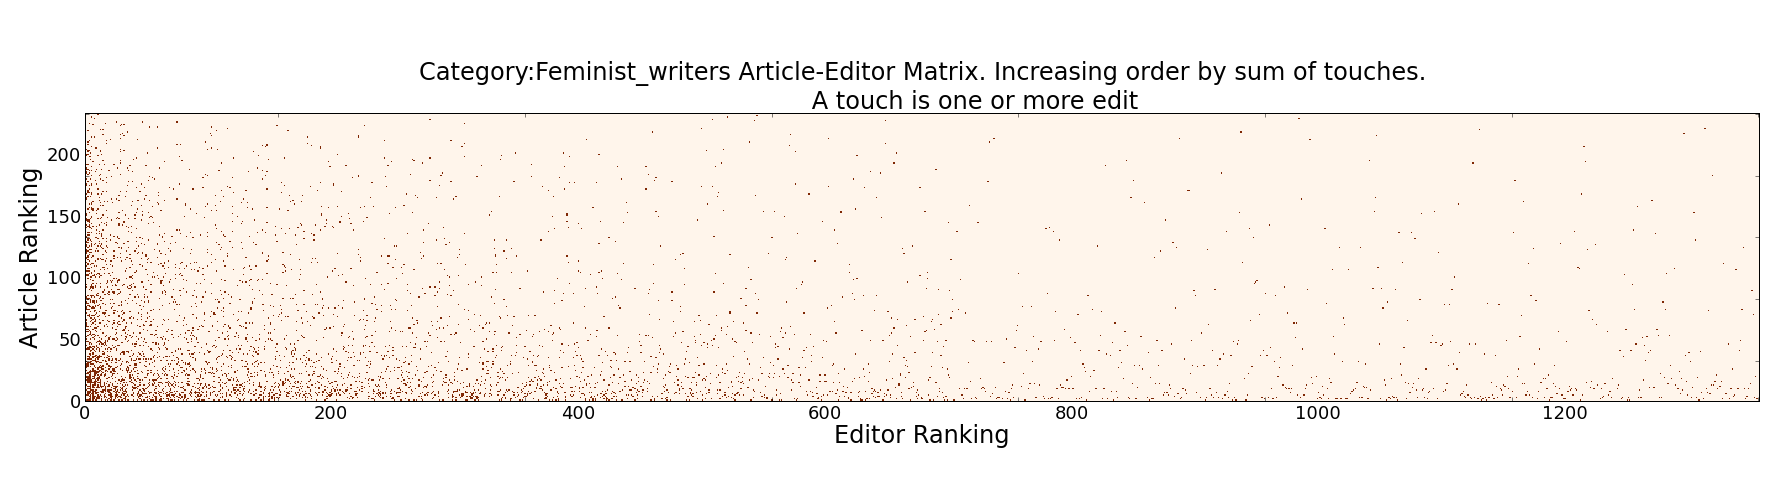
\includegraphics[width=2.0\columnwidth]{../Figures/Category_Feminist_writerstriangle_matrix_corrected.png}
\caption{Typical $\mathbf{\mathit{M_{ea}}}$ matrix for a Wikipedia category (here, {\it Feminist Writers}) ordered on both dimensions by descending order of number of articles modified by an editor (horizontal axis) and of number editors who have modified an article (vertical axis). The structure of $\mathbf{\mathit{M_{ea}}}$ is triangular and shows that some editors have a pervasive activity over articles, while most editors edit only a few. Similarly, some articles receive widespread attention by editors, while most articles are modified only by a few editors.}
\label{fig:triangle}
\end{figure*}

Given $M_{ea}$, the simplest, and arguably naive, way to assess the contribution value (i.e., the {\it expertise} thereafter) of an editor is obtained by summing the number of articles ever edited out of all articles in a category. Similarly, a simple {\it quality} measure for an article is the sum of editors who have ever modified it, following the famous adage on open source development: ``Given enough eyeballs, all bugs are shallow" \cite{raymond1999}. These crude expertise and quality metrics for editors and articles, respectively  given by,

\begin{equation}
\begin{cases}
 w_{e}^{(0)} = \sum_{a=1}^{N_{a}} M_{ea} \equiv k_e\\[7pt]
 w_{a}^{(0)} = \sum_{e=1}^{N_{e}} M_{ea} \equiv k_a
\end{cases}
\label{HHinit}
\end{equation}

are the zero\textsuperscript{th} order of our algorithm. They are the initial step of the {\it method of reflections} proposed by Hidalgo et al., which derives the value of producing entities (i.e., editors) from products (i.e., articles), and {\it vice versa} \cite{hidalgo2007,hidalgo2009}. To help capture the intuition behind the method of reflections for open collaboration, we walk through the first and second iterations:

\begin{itemize}
  \item {\bf 1\textsuperscript{st} order iteration,}  
  \begin{itemize}
  \item {\bf Articles}: if an article has been edited by higher expertise editors, it is of higher quality. That is, quality is a function of expertise calculated from zero\textsuperscript{th} iteration expertise scores.
  \item {\bf Editors}: conversely, if an editor has contributed to higher quality articles, her expertise is higher. That is, expertise is a function of quality calculated from zero\textsuperscript{th} iteration quality scores.
  \end{itemize}
  \item {\bf 2\textsuperscript{nd} order iteration,}
    \begin{itemize}
  \item {\bf Articles}: if an article has been edited by higher expertise editors who have edited higher value articles, which in turn have been edited by higher expertise contributors, the article quality is higher. That is, quality is a function of expertise calculated from 1\textsuperscript{st} iteration expertise scores.
  \item {\bf Editors}: conversely, if an editor has edited higher quality articles, which have been edited by better editors who have edited higher quality articles, then expertise is higher. That is, expertise is a function of quality calculated from 1\textsuperscript{st} iteration quality scores.
  \end{itemize}
 \item {\bf And so on, recursively.}\\
\end{itemize}

Although interpretation is difficult past the very first iteration steps, at each iteration, the algorithm incorporates additional information on the quality of the articles and expertise of editor from the neighboring nodes in the bi-partite network. The higher order iterations 
%of the method of reflections are written as,
%
%\begin{equation}
%\begin{cases}
% u_{e}^{(n+1)} = \frac{1}{k_{e}}\sum_{a=1}^{N_{a}} M_{ea} \, u_{a}^{n}\\[7pt]
% u_{a}^{(n+1)} = \frac{1}{k_{a}}\sum_{e=1}^{N_{e}} M _{ea}\, u_{e}^{n}\\
%\end{cases}
%\label{HHhigher}
%\end{equation}
%
% variable weights to the scores from the previous iteration
can be modeled as a Markov process of random walkers on a bi-partite network, jumping with some probability from one node type to another node type \cite{caldarelli2012network}. A schematic representation of the random walk process on a bi-partite network is depicted in Figure \ref{fig:jumpers}. The intuition is the following: a random walker jumps with some probability from an editor to a given article (i.e., the editor's expertise is positively influenced by the article's quality), and with another probability from an article to a given editor (i.e. the value of the article is positively by the editor's expertise). The binary matrix $M_{ea}$ determines whether a jump between each pair of nodes is possible: if two nodes $e$ and $a$ are not directly connected ($M_{ea} = 0$), the transition probability is 0. Conceptually, the {\it bi-partite network random walker} model is an extension of the single node type (i.e. Web pages) {\it Page Rank} Google search algorithm \cite{page1999pagerank,kleinberg1999} to two types of nodes.

\begin{figure}[!t]
\centering
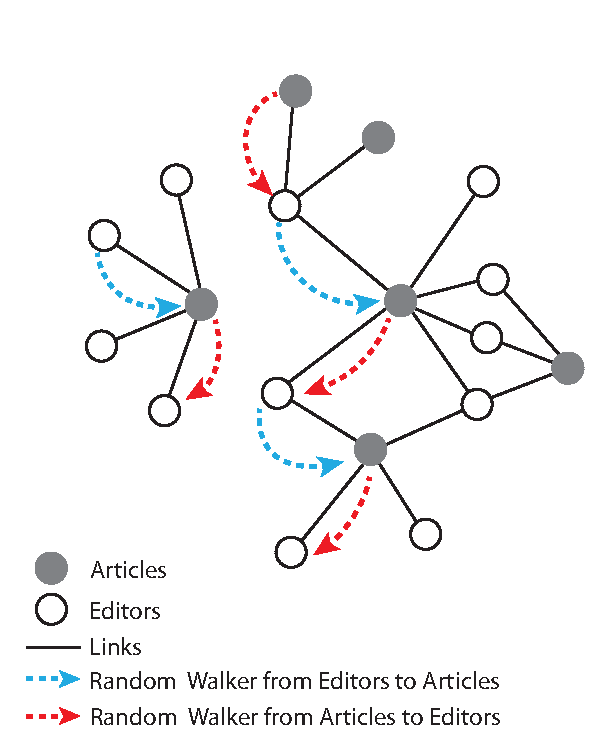
\includegraphics[width=0.7\columnwidth]{../Figures/bi-partite_net.eps}
\caption{Representation of random walkers jumping from editors to articles (red dotted arrows) and from articles to editors (blue dotted arrows). The intuition is the following: a random walker jumps with some probability from an editor to a given article (i.e., the editor's expertise is positively influenced by the article's quality), and with another probability from an article to a given editor (i.e., the value of the article positively influences the editor's expertise).}
\label{fig:jumpers}
\end{figure}

%According to  Caldarelli et al. \cite{caldarelli2012network}, we reformulate the method of reflections to account for jumps of the random walker on the bi-partite network of editors and articles. 
We call $w^{(n)}_e$ the expertise of an editor and $w^{(n)}_a$ the quality of an article at the $n^{th}$ iteration, and we define the following Markov process on the bi-partite network of collaboration, 

\begin{equation}
\begin{cases}
w^{(n+1)}_e (\alpha,\beta) = \sum_{a=1}^{N_a}  G_{ea}(\beta) \,w^{(n)}_a (\alpha,\beta)\\[7pt]
w^{(n+1)}_a (\alpha,\beta) = \sum_{e=1}^{N_e}  G_{ae}(\alpha) \, w^{(n)}_e (\alpha,\beta)\\
\end{cases}
\label{random_walker}
\end{equation}

with $G_{ea}$ the probability  to jump from article $a$ to editor $e$ in a single step, and the probability $G_{ae}$ to jump from editor $e$ to article $a$ also in a single step. These transition probabilities are given by,

\begin{equation}
\begin{cases}
G_{ea}(\beta) = \frac{M_{ea} k_{e}^{-\beta}}{\sum_{e' = 1}^{N_e} M_{e'a} k_{e'}^{-\beta}}\\[10pt]
G_{ae}(\alpha) = \frac{M_{ea} k_{a}^{-\alpha}}{\sum_{a' = 1}^{N_a} M_{ea'} k_{a'}^{-\alpha}}.\\
 \end{cases}
\end{equation}

The transition matrices $G_{ea}(\beta)$ and $G_{ae}(\alpha)$ depend only on the initial conditions: the binary matrix $M_{ea}$, as well as $k_e$ and $k_a$ given by (\ref{HHinit}), and are controlled only by parameters $\alpha$ and $\beta$.  We shall therefore explain only how $\beta$ influences the probability to jump from an article to an editor (i.e. the value of the article positively influences the editor's expertise). For $\beta = 0$, we recover the zero\textsuperscript{th} order iteration (\ref{HHinit}). For $\beta > 0$, the probability to jump from article $a$ to editor $e$ is a power law function $\sim 1/k_{e}^{~\beta}$ of the sum of articles $k_{e}$  modified by editor $e$. Hence, the larger $k_{e}$, the lower the probability to jump from $a$ to $e$ relative to other editors. On the contrary, if $\beta < 0$ the probability to jump from an article to an editor is a positive function of the sum of articles modified by the editor. For $-1 < \beta < 0$, the function is concave, while for $\beta < -1$, the function is convex, which means that the more articles have been edited by the editor, the even more the positive influence on articles. In a nutshell, $\beta$ relates the amount of articles edited on the overall editor's expertise. %which in turn has an influence on each edited article (along with the influence of other editors).
If $\beta \gg 0$, the positive influence of the number of contributed articles on the editor's expertise decreases. If $\beta$ close to $0$, the number of contributed articles increases linearly the editor's expertise. The same considerations hold for $\alpha$ and the probability $G_{ae}(\alpha)$ to jump from an editor to an article (i.e. the expertise of the editor positively influences the quality of an article).

%After each iteration, we have expertise and quality scores, which allow for the ranking of editors and articles respectively. When the rankings for both editors and articles do not change in two successive iterations we consider that the {\it bi-partite network random walker} model has converged. We have verified that the method converges on all our 12 Wikipedia categories.  
Figure \ref{fig:convergence} shows the evolution of expertise $w_e$ ranked among editors having contributed to articles in the {\it Feminist Writers} category on Wikipedia for the set of control parameters $(\alpha,\beta) =(0, 0.72)$. We can see how the algorithm progressively ranks editors: some editors with initial low rank (i.e. with few articles edited), get a higher rank as more information is incorporated from neighboring nodes as the number of iterations increases. In that case ($\beta >0$), higher ranked editors have edited and contributed to fewer, but higher quality articles (i.e. articles edited by more editors who have edited less articles). Similarly, some initially high ranked editors, gradually drop in the ranking. They have edited many, but lower quality articles. 

\begin{figure}[!t]
\centering
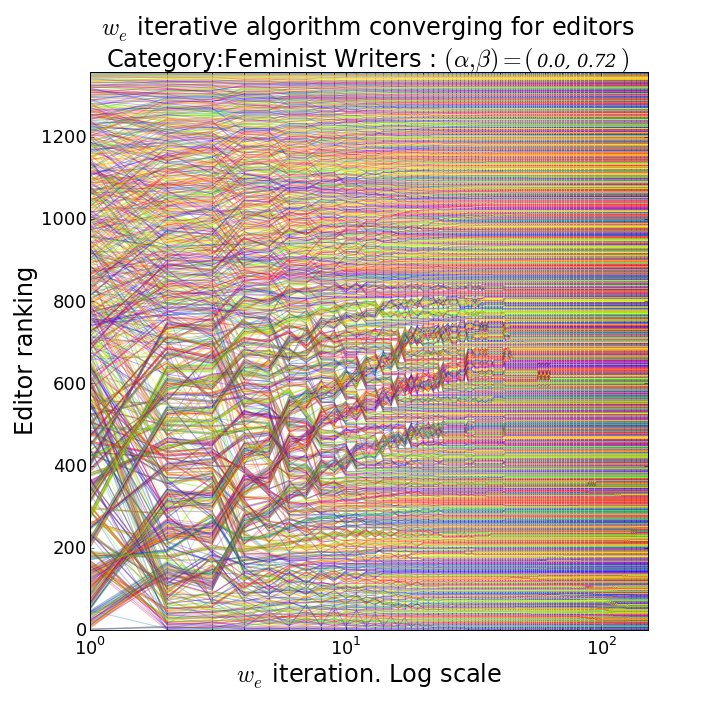
\includegraphics[width=0.9\columnwidth]{../Figures/fem_editors_iter_converge.png}
\caption{Convergence of the ranked expertise $w_e$ of editors having contributed to articles in the Feminist Writers category on Wikipedia for arbitrary control parameters: $\mathbf{(\alpha,\beta) =(0, 0.72)}$. Starting from the sum of contributed articles as the initial step, we can see how the algorithm progressively ranks editors: some editors with initial lowest rank, i.e., with few articles edited, get a higher rank as the number of iterations increases. Similarly, some initially high ranked editors, gradually drop in the ranking. In the case {\it Feminist Writers}, the algorithm converges after $\mathbf{64}$ iterations.}
\label{fig:convergence}
\end{figure}

Upon calibration of the bi-partite random walker model with ground-truth metrics of article quality and editor expertise, the parameters $\alpha$ and $\beta$  directly inform how coordination generates value (i.e. more articles edited by more editors brings value), or on the contrary, if value is created by small clusters of highly experienced editors. This latter scenario implies less coordination among large crowds of contributors.

% describe how editors and articles influence each other at the level of the whole bi-partite collaboration network.
%\textcolor{red}{We cannot calibrate and test because each category is different}
%Whenever calibration shows that the evolution of $\alpha$ and $\beta$ can be predicted, then editor expertise and article quality can also be predicted up to statistical errors. 
%Here, we explain the calibration steps for$\alpha$ and $\beta$ and how the control parameters inform on the structure of value creation in open collaboration. We also document the evolution of these parameters as Wikipedia categories get increasingly enriched with new contributions.
%A property of this algorithm, is that with the following balance condition,
%
%\begin{equation}
%\mathbf{G}_{ae} \mathbf{w}^*_e = \mathbf{G}_{ea} \mathbf{w}^*_a
%\end{equation}
%
%which can be rewritten as,
%
%\begin{equation}
%\begin{cases}
%\mathbf{w}^{*}_{e} \sim \mathbf{k}^{1-\beta}_{e} \langle \mathbf{k}_{a}^{-\alpha}\rangle_e \\
%\mathbf{w}^{*}_{a} \sim \mathbf{k}^{1-\alpha}_{a} \langle \mathbf{k}_{e}^{-\beta}\rangle_a
%\end{cases} \label{eqsim}
%\end{equation}
%
%it is the analytical formulation we use onwards. It is important to note a crucial difference in the way we apply the weighted random walk model in the case of open collaboration compared to the countries-products problem. In \cite{caldarelli2012network}, $w^*_p$ is a measure of ubiquity (i.e. dis-quality) because many countries can sell the product, while here $w^*_a$ is also a measure of ubiquity in the sense that many editors have modified the article. In the case of open collaboration, $w^*_a$ is a measure of quality.

\section{Data}
To uncover the coordination features of Wikipedia categories, we seek to calibrate the bi-partite random walker model with empirical data. For that, we aim to find values of $\alpha$ and $\beta$, which minimize the distance between rankings, of both article quality and editor expertise, given by the model on the one hand, and on the other hand, by ground truth metrics obtained independently. We performed the model calibration for 13 snapshots (see Figure \ref{fig:snapshots})  for each of  the 12 categories of Wikipedia articles presented in Table \nolinebreak \ref{tab:statistics}. To account as much as possible for collaboration structures, we have selected a spectrum of categories ranging from anarchy and edit-warring (e.g., {\it Sexual Acts}) to acknowledged high organization level (e.g., {\it Military history of the US}).

For each category and snapshot we have built the binary matrix $M_{ea}$ by parsing all edit histories of all articles in the main namespace up to the snapshot time. We set $M_{ea} = 1$ for editor $e$ having modified article $a$, and $M_{ea} = 0$ otherwise. We considered only editors who made 5 or more edits to any article in the category. We also discarded all software robots (i.e., {\it bots}) that programmatically edit Wikipedia. 

\begin{table}
\begin{tabular}{|l|c|c|c|}
%\toprule
\hline
{\bf Category} &  {\bf Articles} &  {\bf Editors} &  {\bf Edits} \\
%\midrule
\hline
American male novelists               &      2,460 &   9,946 &  224,783 \\
2013 films                            &      1,896 &   5,215 &  150,956 \\
American women novelists              &      1,936 &   5,968 &  138,716 \\
Nobel Peace Prize laureates           &       104 &   4,165 &   91,522 \\
Sexual acts                           &        93 &   2,190 &   45,901 \\
Economic theories                     &       212 &   1,145 &   28,658 \\
Feminist writers                      &       233 &   1,357 &   25,738 \\
Yoga                                  &       123 &    730 &   25,315 \\
Military history of the US &       180 &    854 &   20,172 \\
Counterculture festivals              &        66 &    578 &   10,515 \\
Computability theory                  &        92 &    272 &    7,117 \\
Bicycle parts                         &        70 &    210 &    4,981 \\
\hline
\end{tabular}
\caption{Size statistics of investigated Wikipedia categories sorted by total edits.}
\label{tab:statistics}
\end{table}

\begin{figure}[!t]
\centering
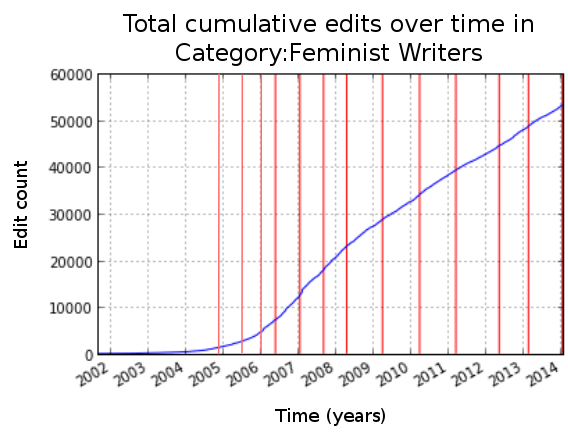
\includegraphics[width=0.9\columnwidth]{../Figures/cumulative_snapshots_Feminist_Writers_thirteen.png}
\caption{Cumulative edits made in Category {\it Feminist writers} (blue line). Vertical red lines represent the 13 snapshots taken at 2.5\%, 5\%, 7.5\% and then, 10\%, 20\%, 30\%, \ldots , 100\% of edits.}
\label{fig:snapshots}
\end{figure}

%\subsection{Editors Expertise and Articles Quality}
To calibrate $\alpha$ and $\beta$, we resorted to state-of-the-art ground truth evaluations for editor expertise $\bar{w}_e$ and article quality $\bar{w}_a$. From these exogenous evaluations, we ranked editors and articles according to their expertise and quality respectively. We then performed  a grid search for values of $\alpha^*$ and $\beta^*$, which maximize the Spearman rank-correlation $\rho_e$ and $\rho_a$ between rankings obtained from the bi-partite random walker model $(w_e,w_a)$ and from exogenous metrics $(\bar{w}_e,\bar{w}_a)$. Actually, $(\alpha^*,\beta^*)$ must maximize both $\rho_e$ and $\rho_a$, even though $\rho_e$ and $\rho_a$ might actually be different. The optimization function  of $(\alpha^*,\beta^*)$ is given by,

\newcommand{\argmax}{\arg\!\max}

\begin{equation}
\begin{cases}
(\alpha^*,\beta^*) = \argmax_{\alpha, \beta}(\rho_e)\\
(\alpha^*,\beta^*) =\argmax_{\alpha, \beta}(\rho_a).\\
\end{cases}
\end{equation}

The set $(\alpha^*,\beta^*)$ characterizes how the structure of collaboration creates values in each Wikipedia category. To calibrate the model, we have used ground truth metrics for article quality and editor expertise. 

A variety of techniques for measuring article quality have been proposed, from a collection of word-count related metrics \cite{blumenstock2008sizematters} to analyzing persistent and transient contributions throughout revisions \cite{woehner2009}. We have selected metrics used on Wikipedia \cite{wang2013tell,klein} which have also been used in the CSCW literature in different combinations \cite{kane2011,keegan2012}. Our measure of actual article quality is a combination of 5 text analysis metrics: (i) ratio of mark-up to readable text, (ii) number of headings, (iii) article length, (iv) citations per article length, (v) number of outgoing intra-Wiki links. We performed principal component analysis (PCA) for each category and snapshot in order to reduce dimensionality from 5 metrics to a single one (i.e., the principal component). The variance explained by the principal component varied between 0.5 and 0.72, confirming the dominance of the axis of maximum variance. Even though these five article quality metrics do not directly incorporate information from the bi-partite network (e.g. number of contributors, number of edits), they might indirectly be related, as some editors specialize in some types of editing, such as adding citations or systematically improving the structure of articles.

Editor expertise is even more difficult to address. As each article is a blend of edits by several contributors, disentangling the value of individual contributions remains a challenge, which has occupied Wikipedia researchers long before us. Techniques ranging from parsing the revision history to measuring text survival rate \cite{adler2008measuringauthor} have been used. Although they are sophisticated, these metrics pose a variety of problems. For instance, some articles are likely to evolve not only because former editors introduced wrong statements, but simply because of new information brought to public attention. 

We decided to use the {\it labor hours} metric proposed by Geiger and Halfaker \cite{geiger2013}, which is calculated for each editor by taking contribution history up to the snapshot point. All edits made within $1$ hour of a previous edit are counted as one {\it edit session}. If more than one hour separates two edits, a new period of edits  starts. The expertise expressed in labor hours is the sum of edit sessions. For the calculation of ground truth expertise, we only consider edits for a given category, although the same editor might have simultaneously  edited other categories of Wikipedia. This metric purposefully does not tell how this time is spent in the number (resp. size) of edits actually made during a period, or whether the effort has been spent on one or multiple articles. In other words, we do not distinguish a single minded user spending $100$ hours on a single article trying to get it to ``feature article status" from a user making $100$ stub articles for $1$ hour each.  However, it is clear that a highly contributing editor has more chance to touch more articles over time, but the metric does not distinguish if editors had a dispersed contribution or concentrated on a single article. 

How this effort is distributed and brings quality is precisely what the {\it bi-partite random walker} model can say that other metrics cannot. In a nutshell, parameters $\alpha$ and $\beta$ describe the most likely structure of collaboration given calibration of the model to ground truth quality and expertise metrics. The higher the correlation between the model and the exogenous metrics, the better the collaboration structure is captured by the model. 

%Finally, we shall discuss shortly the possibility that ground-truth article quality and editor expertise might be dependent. For instance if one category was just much easier to write about and the average editor was simply better at writing about it. Well in fact these are the criticisms of the biases of Wikipedia, that it has a very specific male, global north, young, technological demographic. That is why we attempted to mix categories which would play into this systemic bias (like Computability and Economic theory), with those that would be neglected by such bias (like Feminist Writers and Yoga). Clearly this is a stereotypical approach, but at least we will be able to view some variance. 

% \textcolor{red}{Yet depending on our amount of preferential attachment in our network, one or the other could be seen as a superior editor. Likewise on pages, an article text can be changed in 5 ways. The same edits could be made by one generalist editor or 5 specialist editors, and the ground-truth would not change. Depending on a different preferential attachment parameter in the model could rank each of these very differently.}
%
%\textcolor{red}{Finally a point should be made about whether our exogenous expertise and quality measures are independent. Earlier on links between expert editors and quality articles were claimed \cite{wilkshuber}, and would seem intuitive. Yet, subsequently, there have been claims against such universal links which point out that key social interactions are not accounted for with these measures \cite{kane2009}. Intuitively this link rests on the collaborativeness of the articles and editors in question. With collaboration expertise will transtlate into article quality. However, given antagonistic, warring- editors expertise will not improve article quality.}

\section{Results}
To understand how contributions by editors to articles shape the structure of collaboration in Wikipedia, we have performed a calibration of the bi-partite network random walker model on 12 Wikipedia categories (c.f., Table \ref{tab:statistics}) with 13 snapshots each (Figure \ref{fig:snapshots}). For each category and snapshot, we found the set of parameters $(\alpha^*,\beta^*)$, which maximize the fitness of the model to ground truth metrics of article quality and editor expertise. Figure \ref{fig:landscape} shows typical optimization landscapes, which maximize the rank correlation $\rho_e$ (upper panel) between editor expertise $w_{e}$ obtained from the model and expertise obtained from ground truth measures $\bar{w}_e$. The same is done for rank correlation $\rho_a$ between $w_a$ and $\bar{w}_a$ (lower panel). 

\begin{figure}[!t]
\centering
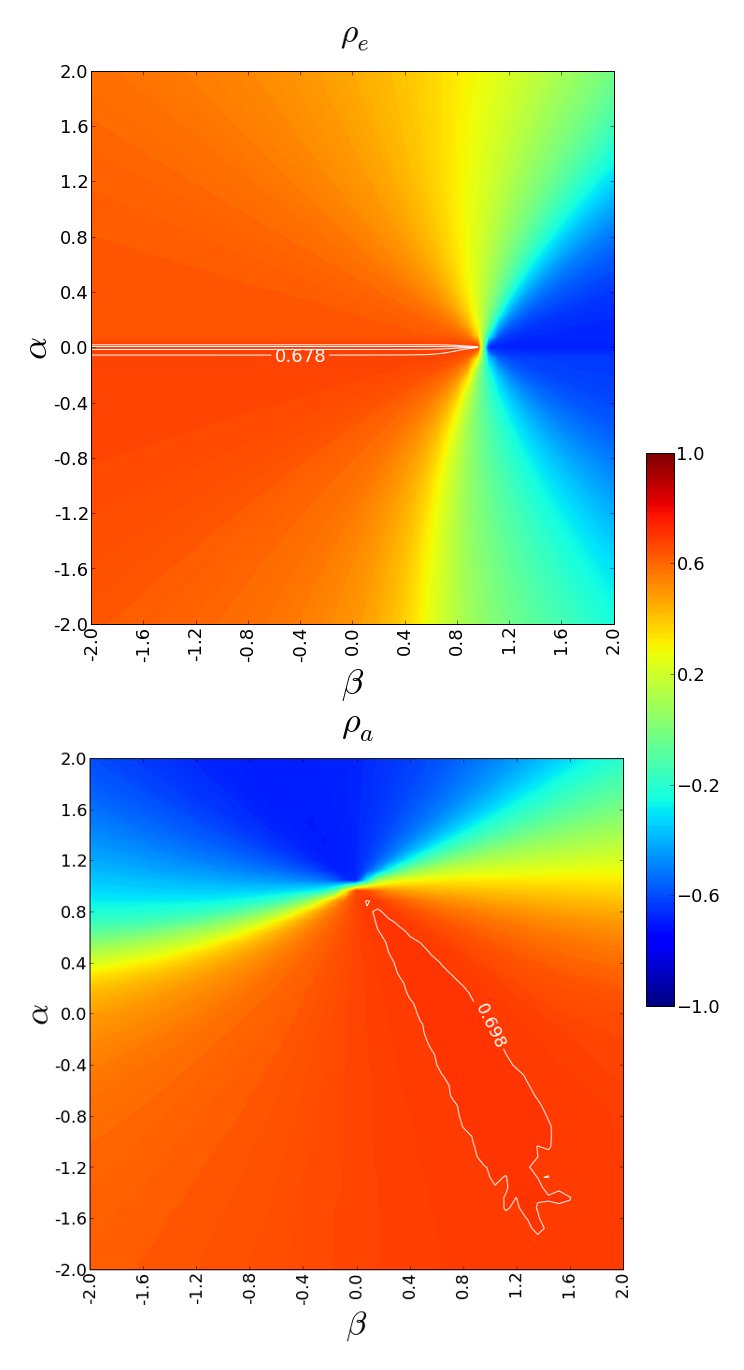
\includegraphics[width=0.9\columnwidth]{../Figures/contour_fem_combined.png}
\caption{Typical landscape of maximum correlation as a function of $\alpha$ and $\beta$ for articles (upper panel) and editors (lower panel). The contour line shows the 95\textsuperscript{th} percentile of the rank correlation over the landscape. The category displayed here is {\it Feminist Writers}, for the last snapshot ending February 2014.}
\label{fig:landscape}
\end{figure}

The maximum achievable rank-correlation with ground truth expertise and quality metrics for editors \cite{geiger2013} and articles \cite{wang2013tell} shows that the bi-partite network random walker model accounts particularly well for both quality of articles ($0.58 < \rho_a < 0.91$) and expertise of editors ($0.46 < \rho_e < 0.75 $) at the last snapshot. Actually, the model reproduces very well, and very early the ranking of editors and articles according to the ground truth metrics as shown on Figure \ref{fig:rhotime}. In particular, the quality of articles is very well accounted for, while the level of correlation with the ground truth of editor expertise exhibits a slightly concave, or at least linear, increase.

%The question remains if the intersection of the solution spaces for $\rho_a$ and $\rho_e$ is nonempty. That is whether the we can find values of $\alpha$ and $\beta$ for which our editor ranking and article ranking are simultaneously optimized. We exploit two empirical facts from our data: the clear solution for article rankings that $alpha = 0$, and that for editor rankings the 95\textsuperscript{th} percentile maximizing boundary always includes values at $\alpha = 0$. Therefore, with $\alpha = 0$, we solve for $\beta$ in the editor ranking that maximizes $\rho_e$ - and thus $\rho_a$ simultaneously. 

For the latest snapshot (i.e., the state of contributions in February 2014), we find that the best possible $\alpha^*$ is $0$ in all circumstances, while $\beta^*$ varies considerably across categories. Table \ref{tab:maxbeta} shows the categories ordered by $\beta^*$ (and $\alpha^*=0$ for the sake of completeness), as well as the corresponding maximum rank correlations $\rho_e$ and $\rho_a$. Since there is no single optimal value for $(\alpha^*,\beta^*)$, but rather a space of optimal values for  $\rho_e$ and $\rho_a$ separately, we have searched for a set of values that jointly maximizes both $\rho_e$ and $\rho_a$. The optimal parameter $\alpha^* = 0$ means that editor expertise always benefits from contributions as a linear function of the number of articles edited [compounded over iterations of the recursive algorithm defined by formula (\ref{random_walker})].  However, $\beta^*$ exhibits a continuum of values between $0$ ({\it Bicycle parts} and {\it US Military History}) and $1.52$ ({\it Sexual Acts}). $\beta$ controls the influence of the number of editors on the quality of a given article. When $\beta \approx 0$, the quality of articles increases as a linear function of the number of editors who have modified them. For $\beta \gg 0$, the marginal gain of having more editors for a given article decreases. So, in that case, when the number of editors touching an article increases, the marginal quality improvement decreases.

The evolution of $\beta^{*}$ over snapshots as shown on Figure \ref{fig:rhotime} exhibits large variations for early snapshots corresponding to the early 10\% of overall contributions per category (i.e., the 4\textsuperscript{th} snapshot). While $\beta^{*}$ exhibits a tendency to more stability afterwards, large variations within the range $0$ to $1.5$ can be observed for some categories, suggesting that organization and coordination level changes can occur as categories develop. 

%In fact, $\beta$ switches signs only 3 times of the possible 144 measured changes. Although there are not enough $\beta < 0$ to draw a firm conclusion, it is interesting to note that instances of $\beta < 0$ happened in early category history, hence suggesting that the early contributions steps pull more value from the community. 
%The stability of $(\alpha^*,\beta^*)$ confirms that the control parameters of the bi-partite network random walker model describe a robust feature of the structure of value creation in the bi-partite network of editors contributing to articles. This additional result is also a first step towards robust predictions of editor expertise and article quality rankings, given successive inputs to new articles made by editors.


\begin{table}
%\end{table}
\begin{tabular}{|llcccc|}
\hline
         &                     Category & $\rho_a$ & $\rho_e$ & $\alpha^{*}$ & $\beta^{*}$ \\
\hline
 1&                        Bicycle parts  &     0.90 &     0.46 &     0.00 &    0.00 \\
 2&Military history of the US  &     0.58 &     0.70 &     0.00 &    0.00 \\
  3&                Computability theory &     0.77 &     0.56 &     0.00 &    0.32 \\
   4&            American male novelists &     0.67 &     0.75 &     0.00 &    0.40 \\
    5&                        2013 films  &     0.72 &     0.55 &     0.00 &    0.48 \\
     6&                Economic theories  &     0.74 &     0.70 &     0.00 &    0.48 \\
     7&         American women novelists  &     0.63 &     0.75 &     0.00 &    0.64 \\
     8&                 Feminist writers  &     0.70 &     0.69 &     0.00 &    0.72 \\
     9&                             Yoga  &     0.64 &     0.57 &     0.00 &    1.12 \\
     10&      Nobel Peace Prize laureates  &     0.91 &     0.66 &     0.00 &    1.20 \\
      11&        Counterculture festivals  &     0.80 &     0.61 &     0.00 &    1.36 \\
        12&                   Sexual acts  &     0.63 &     0.66 &     0.00 &    1.52 \\
\hline
\end{tabular}
\caption{Categories ordered by increasing $\beta^{*}$ obtained from best rank-correlation $\rho_a$ and  $\rho_e$
 of the {bi-partite network random walker} with the ground truth. As shown on the upper panel of Figure \ref{fig:landscape}, highest rank-correlation is always obtained for $\alpha^{*} = 0$ suggesting that editors are experts in direct proportion to the number of articles they edit. The different values of $\beta^{*}$ show the effect of marginal editors on a article. As $\beta^{*}$ grows larger having more editors shows diminishing returns on article quality - ``too many cooks spoil the broth".}
\label{tab:maxbeta}
\end{table}


%However, for categories with $\beta >0$ the quality of an article is also negatively influenced by the portfolio size of its editors. In other words, when $\beta$ is large, the more articles an editor edits, the lower his or her contributed value to one single article. $\beta$ also characterizes each category and the way quality is achieved through the cumulative contribution of information. For $\beta$ small, all editors have a fairly equal chance to contribute positively to any article, while for $\beta$ large, an editor can only contribute positively to a subset of articles (the larger $\beta$ the smaller the set). Typically, it is unlikely for a single person to have visited all {\it counterculture festivals}, performed all {\it sexual acts} or {\it Yoga} practices, while it is easier for anyone to gather relevant information on {\it bicycle parts} or the {\it US military history}. 





%\textcolor{red}{\bf Is there any reshuffling of ranking over time, or do they stay the same?}



\begin{figure}[!t]
\centering
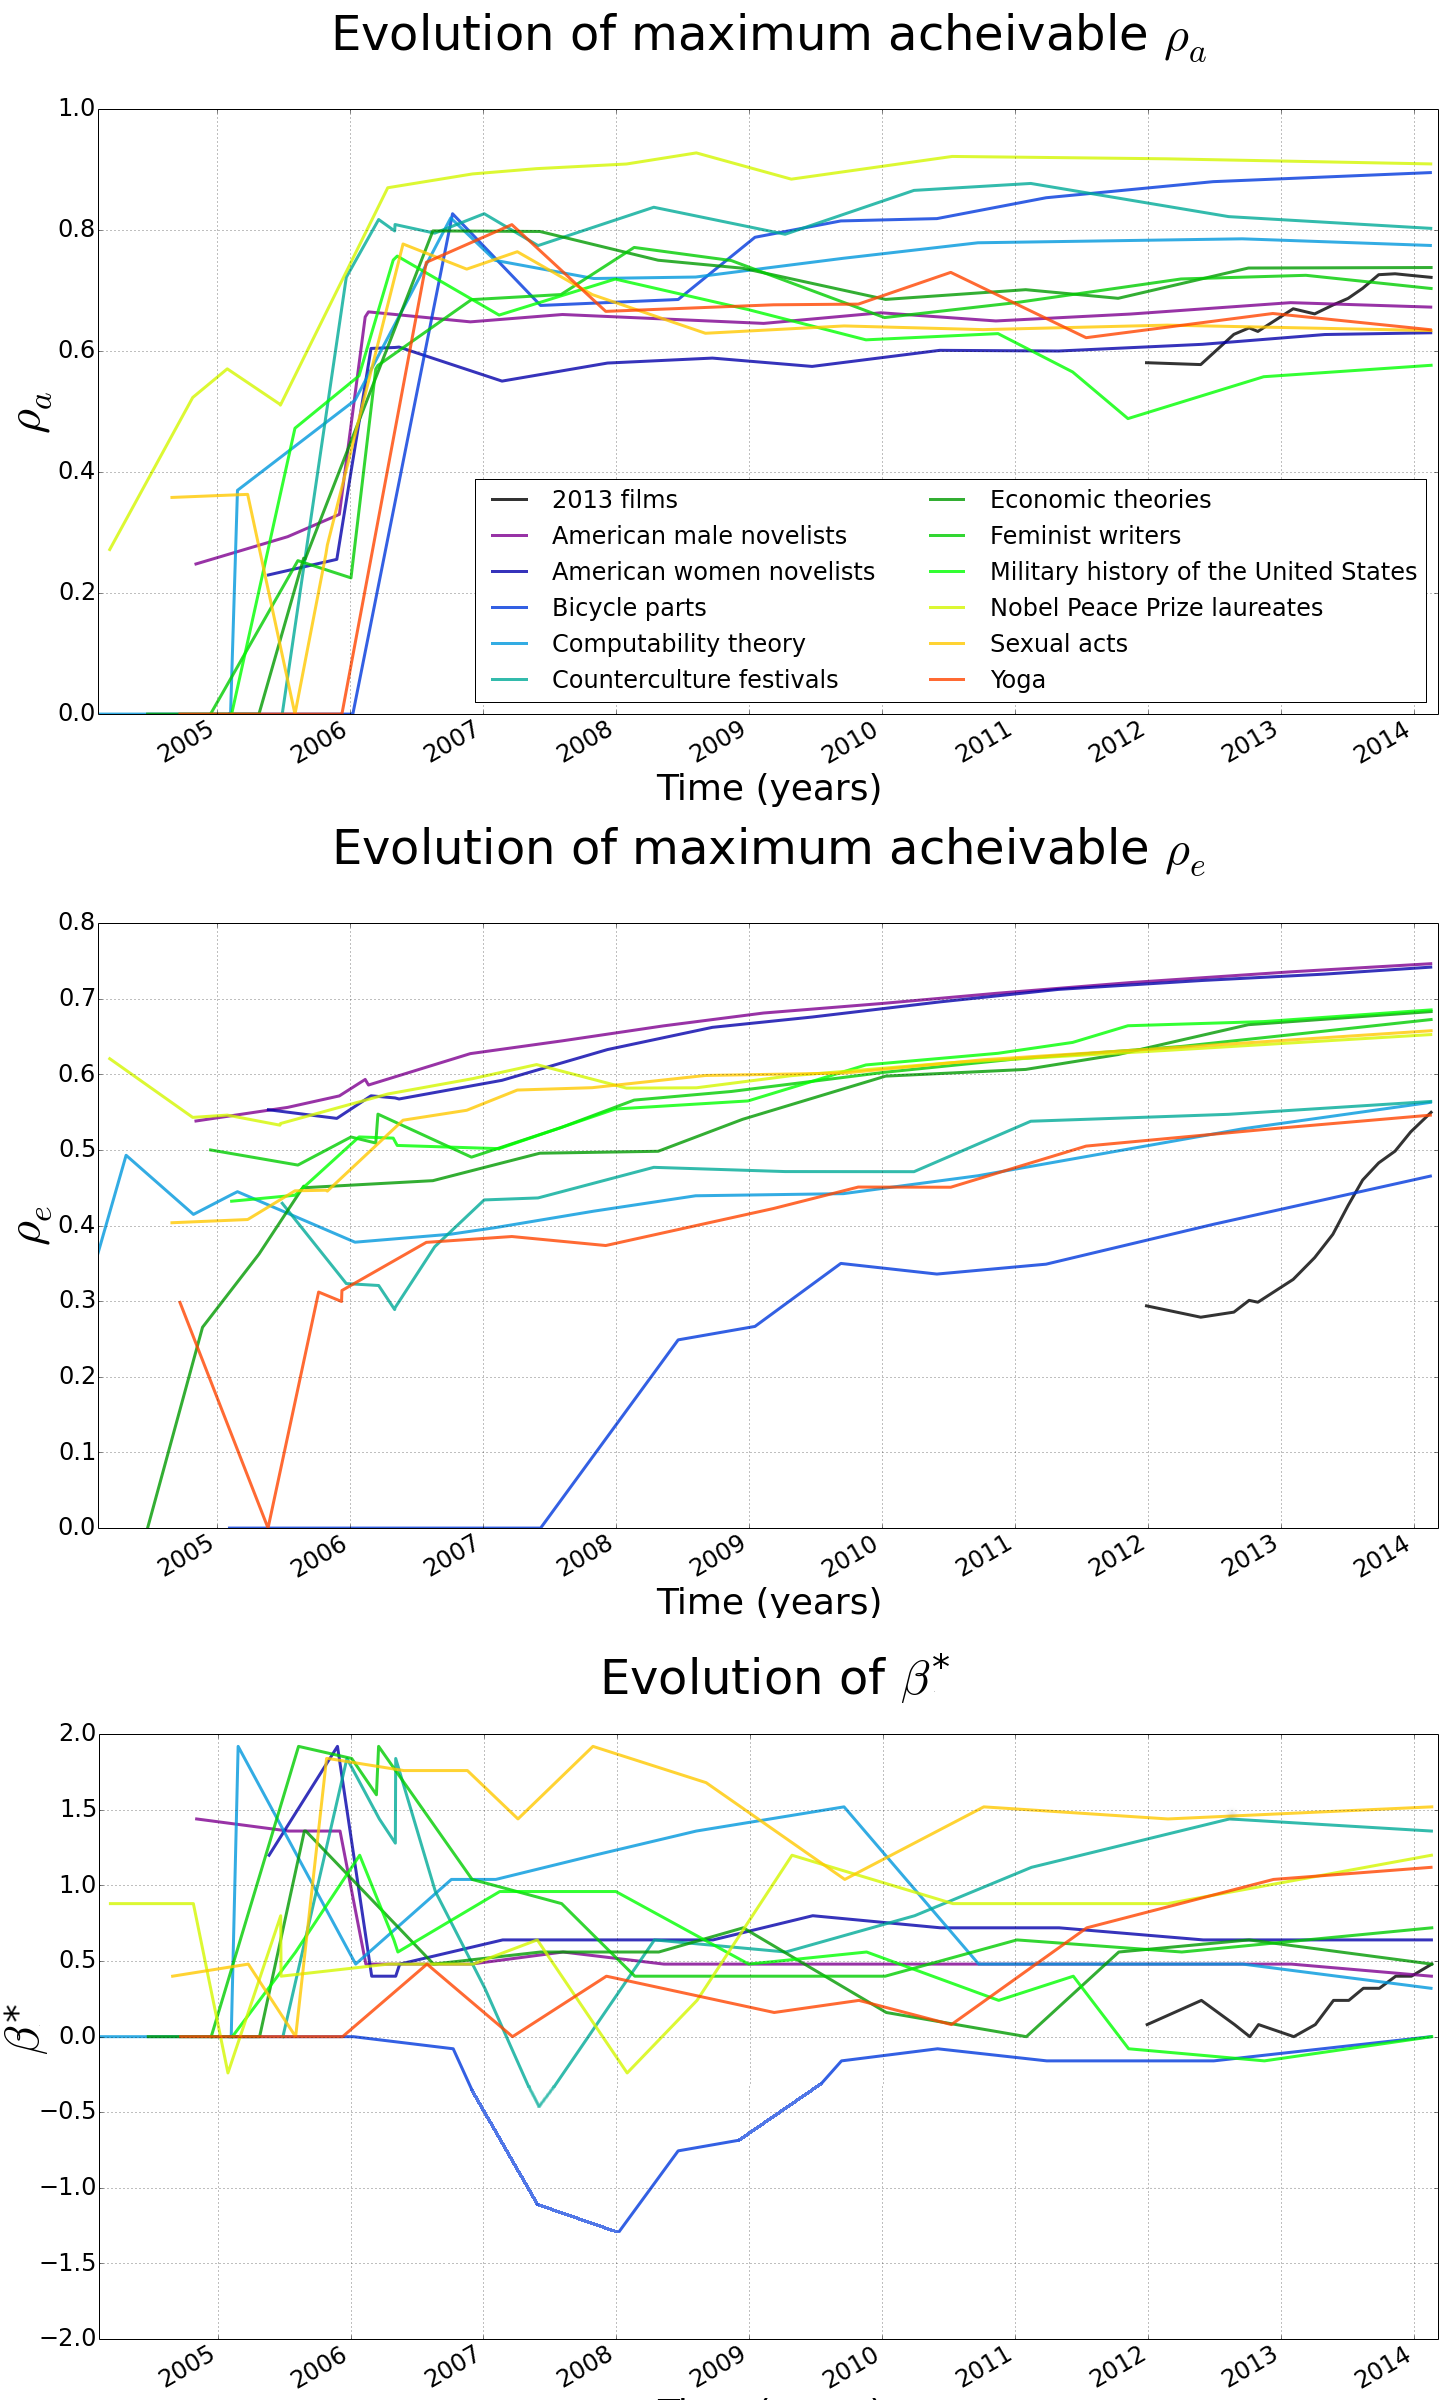
\includegraphics[width=0.9\columnwidth]{../Figures/rho_combined_with_beta.eps}
\caption{Evolution of Spearman $\rho$ rank correlations between the ranking obtained from the calibrated model and the actual values for each category and for editors (upper panel)  and articles (middle panel). Corresponding $\beta^{*}$ values are also shown for interest (lower panel). The correlations are generally quite high : $ 0.46 < \rho_e < 0.75$ with $\langle \rho_e\rangle = 0.64$ for editors and $0.57 < \rho_a < 0.91$ with $\langle \rho_a\rangle = 0.72$. $\rho_{a}$  is stable over time, which means that the quality of articles can be well captured early on by the model. However, $\rho_e$ exhibits a convex increase over time, suggesting that it takes time (i.e., lots of edits) to capture well the expertise of editors.}
\label{fig:rhotime}


\end{figure}

	



\section{Discussion}
To understand how the structure of collaboration influences article quality, we have applied and tested the {\it bi-partite network random walker} model for a variety of categories in Wikipedia. Our results show that the model accounts well for the quality of articles  $\langle \rho_a \rangle  \approx 0.64$ and for the expertise of contributors $\langle \rho_e \rangle  \approx 0.72$, and overall exhibits a high degree of fitness. Moreover, $\rho_a$ remains stable over time, while $\rho_e$ increases, suggesting that the model better reflects editor expertise as more contributions to a broader set of articles occur, i.e., when the bi-partite network gets more densely connected. This suggests that loosely connected entities, either articles and editors, cannot be ranked accurately. From Figure \ref{fig:triangle} and from Table \ref{tab:statistics}, we see that there are always significantly more editors than articles for each category. Hence, the probability for an article to get contributions early on is higher than the probability to find editors who have contributed to a lot of articles early. 

To account for single-minded editors who have concentrated on only one or few articles, we have tested the {\it bi-partite random walker} model with a different input, namely the matrix of edit counts (instead of a binary matrix). As shown on Figure \ref{fig:binary_vs_editcount}, the model using the {\it edit counts} input matrix accounts nearly as well for article quality, while it does a much worse job ranking editor expertise compared to a {\it binary} input matrix. Counter-intuitively, we observe a {\it less is more} situation: the number of articles ever touched by an editor better reflects the structure of collaboration and value creation, compared to edit counts, a much richer information input. Also, the labor-hour ground truth metric for editors is more a proxy of number of edits rather the number of articles ever touched \cite{geiger2013}. Nevertheless, the model does not perform as well with {\it edit counts} as an input. This suggests that what really counts for assessing the expertise of an editor is the number of articles touched, rather than the number of edits per article.

\begin{figure}[!t]
\centering
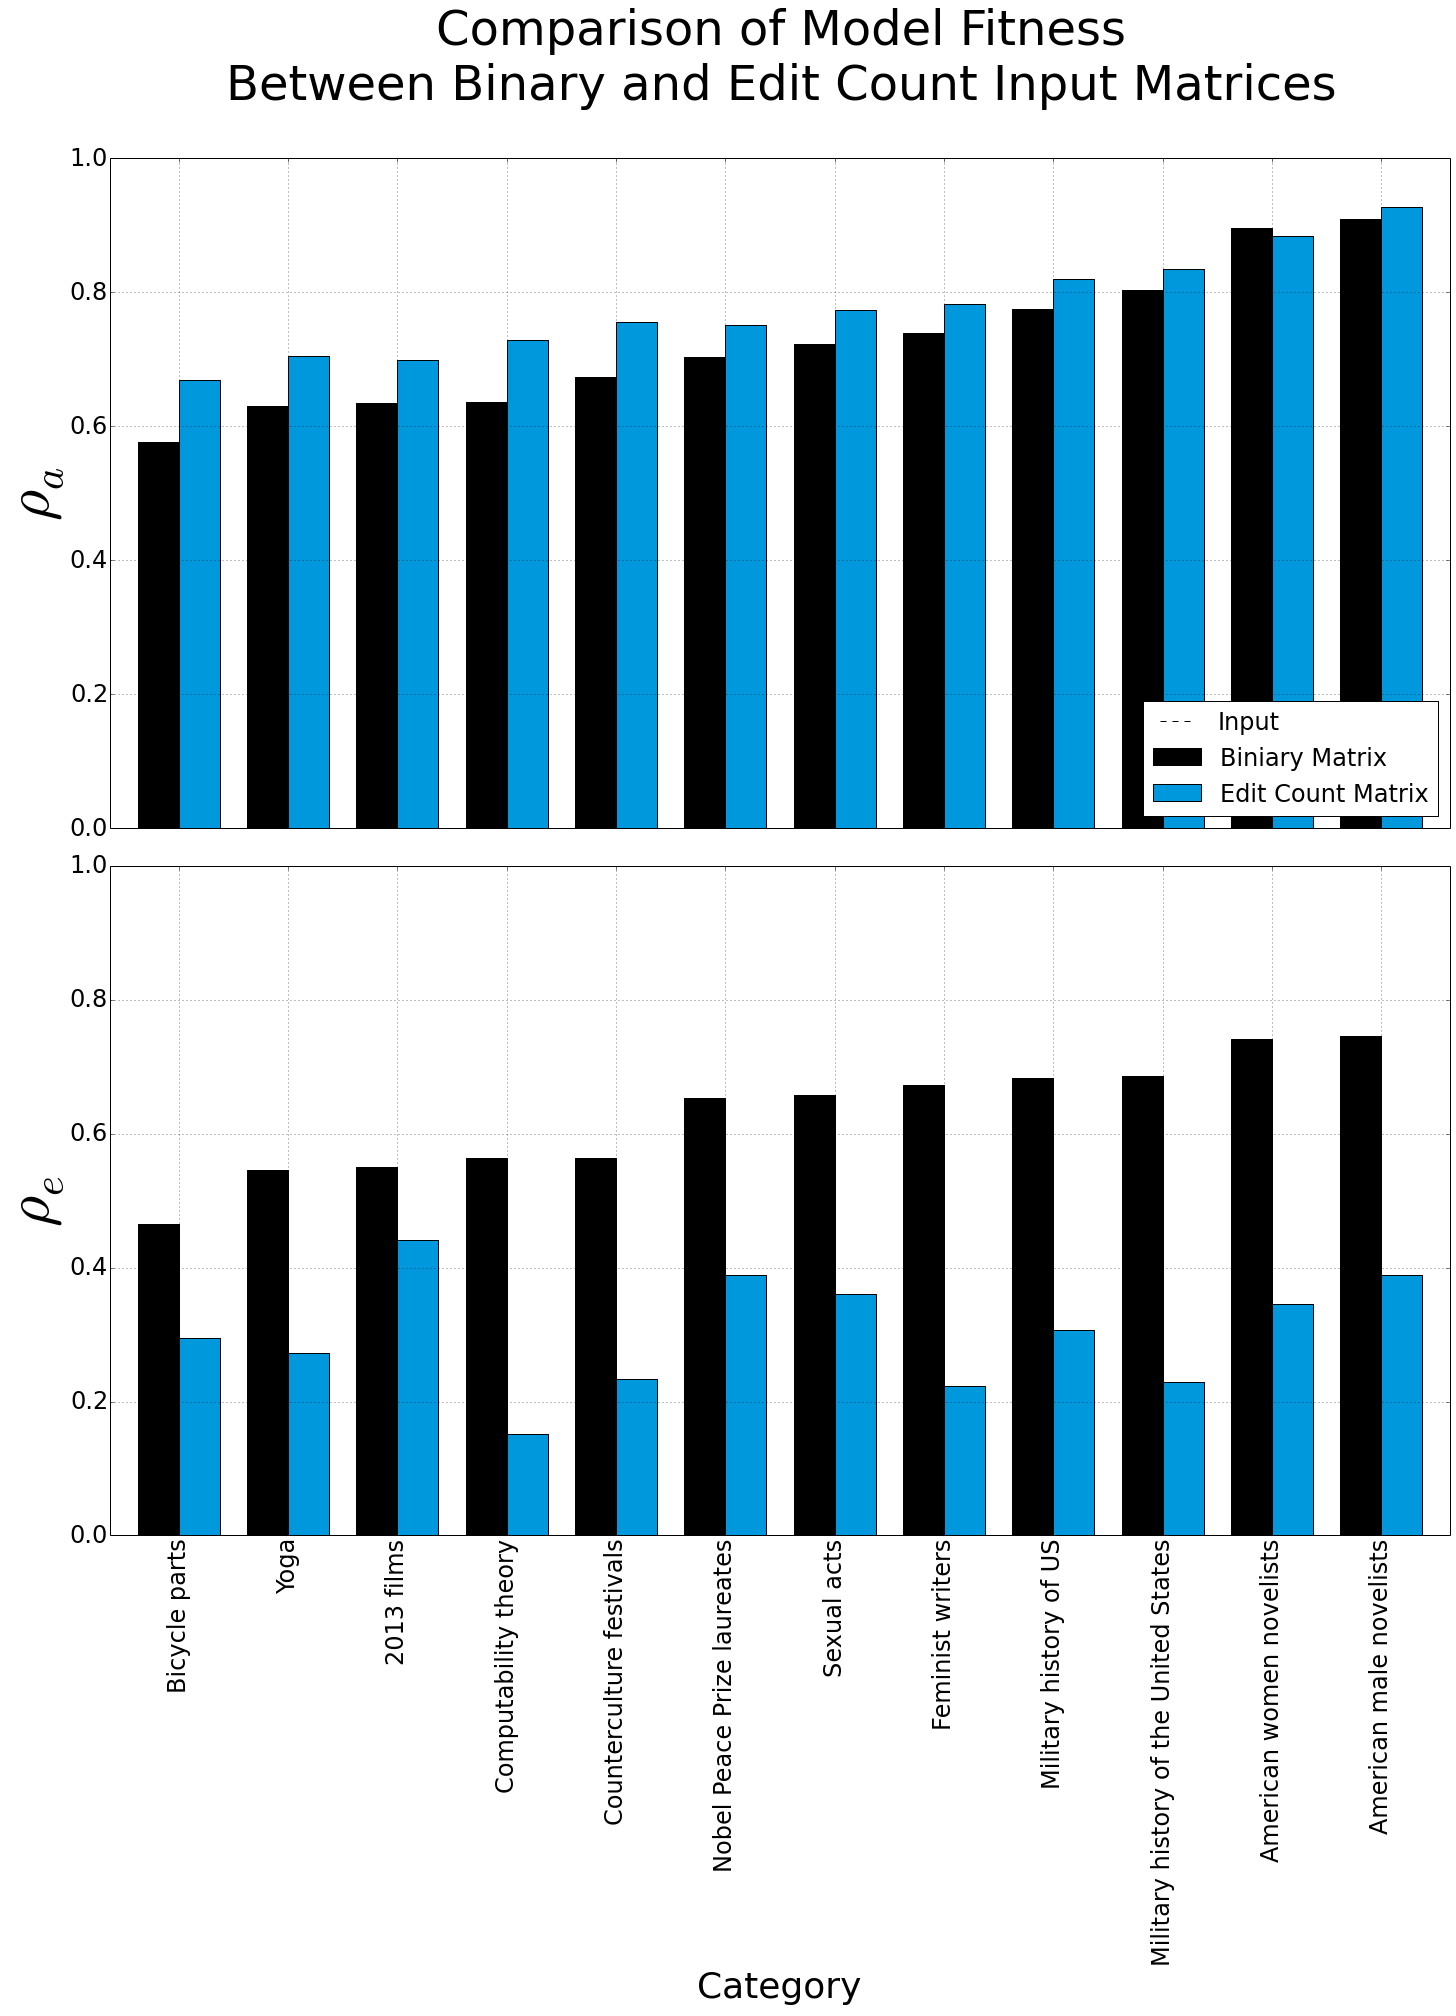
\includegraphics[width=0.9\columnwidth]{../Figures/bin_comp.png}
\caption{Comparison between $\rho_a$ (upper panel) and $\rho_e$ (lower panel) for two input matrices: binary (black) and edit counts (blue) for each category numbered according to Table \ref{tab:maxbeta}. While taking edit counts as the input matrix only marginally increases $\rho_a$, it drastically reduces $\rho_e$.}
\label{fig:binary_vs_editcount}
\end{figure}

We now discuss how the fitted parameters $\alpha^{*}$ and $\beta^{*}$ inform on the structures of collaboration in Wikipedia categories. On the one hand, we have found $\alpha^{*} \approx 0$ for all categories, reflecting the positive influence of the number of articles edited on editor expertise. This result is compatible with previous results by Keegan et al. \cite{keegan2012}. On the other hand, $\beta^{*}$ varies across categories with values ranging from $0$ to $1.52$ at the last snapshot. $\beta$ can be considered as a measure of the collaboration structure: the smaller $\beta$, the more articles benefit from more editors. On the contrary, the larger $\beta$, the more articles benefit from less editors. If we consider for instance {\it Sexual acts}, a category that could be considered taboo or perverse with articles being the least collaboratively edited: $\beta > 1$ reflects that an editor with edits to many articles will see her ranking drop. Indeed, it should not be taken for granted that contributions are necessarily positive. Because of their socially-sensitive nature, articles about sexual acts are particularly prone to attracting vandals or edit-warring behaviors across the whole category. Therefore, editors making the most edits are not necessarily the ones improving article quality, as we would typically expect. This result is again compatible with previous research, which has shown that, in some circumstances, most active editors exhibit deleting behaviors that lower metric-based article quality ratings \cite{kane2011}. 

Conversely, the category {\it Military History of the US} is famous for its self-organized task-forces. At the latest snapshot $\beta = 0$, it is the one of only a few categories we have analyzed, which exhibits $\beta$ consistently negative over time. Accordingly, the marginal quality of articles is positively influenced by the number of editors touching the article. Unsurprisingly, {\it Military History of the US} is literally a {\it WikiProject} with a hierarchy of coordinators, an active IRC channel, and a mailing list. As a result of better coordination, there is less edit-warring and more efficient contributions: editors edit articles with well-defined task at hand. 


%It requires a frictionless, collaborative environment where the more you edit, the more and more experienced you become. It's also worth noting that \cite{keegan2012}, found that ``coordination demands influence the tendency of editors with similar levels of experience to work together". \textcolor{red}{In our scenario that would mean that the coordination present attracts super-users to work in the productive environment. The category Military History is empirically a standout case of collaboration, and shows in its calibrated $\beta$ measurements. }




%This fact tells actually a lot about the model.  The actual metric for editor expertise takes only into consideration the labor hours \cite{geiger2013}, and the more time is spent editing a category, the more likely the editor will have modified a large quantity of articles. The value of $\alpha$ can therefore be explained entirely by the nature of the ground-truth metric. 

%This difference might be due to the roughness of the actual metrics for editors $\bar{w}_e$, expressed in labor-hours, compared to the quality of $\bar{w}_a$, which is an aggregate measure of five precise quality metrics. Nevertheless, the correlation of editor ranking with $\bar{w}_e$ increases: $\rho_e$ exhibits a convex increase over time, suggesting that it takes time (i.e. lots of articles edited) to capture well the expertise of editors. 

%Although it would require further testing with a broad variety of metrics, it seems that the {bi-partite network random walker} model can {\it tune} to whatever ground-truth metric used for calibration. In other words, the values of $\alpha$ and $\beta$ only reflect the structure of value creation in open collaboration, {\it given} the chosen ground-truth metrics. 


% Allowing for a moment, $\alpha = 0$ we can simplify our analytic solutions to gain a more intuitive interpretation of the calibration results.}

% %\begin{cases}
% \begin{equation}
% w^{*}_{e} \sim k_{e}^{1-\beta}\langle k_{a}^{-\alpha} \rangle_{e},\\
% w^{*}_{a} \sim k_{a}^{1-\alpha}\langle k_{e}^{-\beta} \rangle_{a}
% \end{equation}
% %\end{cases}
% 
%Then letting $\alpha = 0$, we can simplify to:
%%\begin{cases}
%\begin{equation}
% w^{*}_{e} \sim k_{e}^{1-\beta}\\[7pt]
% w^{*}_{a} \sim k_{a}
% \langle k_{e}^{-\beta} \rangle_{a}\\[7pt]
% \end{equation}
% %\end{cases} 





%\textcolor{red}{That fact that we find two very different cases of collaborativeness is important in explaining previous contention in computer support collaborative work sphere. Early on, research was release to suggest that high editor inequality among editors is related to high article quality \cite{kittur08}. The intuition is that the top superusers can be unrivaled in shaping the articles. We have certainly found this to be true in the Military History example. Yet later, it was found that editor inequality relating to article quality is unsupported, and editor inequality relating to coordination is false \cite{arazy}. In the case of chaotic categories like Sexual Acts we found this case, where the top users cannot make as much a positive impact as otherwise. These two seemingly contradictory findings can be explained through our measure of collaborativeness. Each part of wikipedia can exhibit different and measurable relationships between editor quality and article quality - that is our collaborativeness $\beta$. }

%$\mathbf{M}$ : most basic measure of collaboration, which represents the bi-partite network contributions to articles by editors: Here, we consider the simplest information available on collaboration: has an editor modified an article at any point in time or not ?


%Analyzing the Creative Editing Behavior of Wikipedia Editors: Through Dynamic Social Network Analysis \footnote{This paper analyzes editing patterns of Wikipedia contributors using dynamic social network analysis. We have developed a tool that converts the edit flow among contributors into a temporal social network. We are using this approach to identify the most creative Wikipedia editors among the few thousand contributors who make most of the edits amid the millions of active Wikipedia editors. In particular, we identify the key category of �coolfarmers�, the prolific authors starting and building new articles of high quality. Towards this goal we analyzed the 2580 featured articles of the English Wikipedia where we found two main article types: (1) articles of narrow focus created by a few subject matter experts, and (2) articles about a broad topic created by thousands of interested incidental editors. We then investigated the authoring process of articles about a current and controversial event. There we found two types of editors with different editing patterns: the mediators, trying to reconcile the different viewpoints of editors, and the zealots, who are adding fuel to heated discussions on controversial topics. As a second category of editors we look at the �egoboosters�, people who use Wikipedia mostly to showcase themselves. Understanding these different patterns of behavior gives important insights about the cultural norms of online creators. In addition, identifying and policing egoboosters has the potential to increase the quality of Wikipedia. People best suited to enforce culture-compliant behavior of egoboosters through exemplary behavior and active intervention are the highly regarded coolfarmers introduced above. }\cite{iba2010}


%{\bf Network Analysis of Collaboration Structure in Wikipedia} \footnote{In this paper we give models and algorithms to describe and analyze the collaboration among authors of Wikipedia from a network analytical perspective. The edit network encodes who interacts how with whom when editing an article; it significantly extends previous network models that code author communities in Wikipedia. Several characteristics summarizing some aspects of the organization process and allowing the analyst to identify certain types of authors can be obtained from the edit network. Moreover, we propose several indicators characterizing the global network structure and methods to visualize edit networks. It is shown that the structural network indicators are correlated with quality labels of the associated Wikipedia articles.} \cite{brandes2009}


%The problem of ranking entities and their respective production is relevant to the flourishing production of knowledge on the Web, and is directly related to two outstanding problems, which have been previously debated. First, how do we gauge the quality (resp. reliability) of blog posts, book reviews (e.g. on Amazon), or restaurant reviews (e.g. on Yelp) ?  Second,  how to grant editing and administrative privileges on community networks (e.g. Slashdot) and on online collaborative platforms (e.g. Wikipedia) \cite{halfaker2013}. 

\section{Limitations and Future Work}
As a two node extension of the {\it pageRank} algorithm \cite{page1999pagerank,kleinberg1999}, the {\it bi-partite network random walker} model is an efficient approach to recursively traverse the complex network of articles and editors in Wikipedia. Our results show that model calibration accounts well with ground-truth metrics, and can help characterize how more contributors for each article and better (resp. less) coordination create value (resp. destroy value) in open collaboration. Its very simple input (a binary matrix of contributions) makes it computationally affordable, though not cheap. While applying this algorithm to the entire Wikipedia would be a challenge, it is straightforward to use on small wikis or most open source software projects.

Our results show a first attempt to understand the structure of cooperation and how value is created with a unique model, which can be fully rationalized. The pertinence of the {bi-partite network random walker} for the study of open collaboration shall be confirmed by future work,  to examine in a systematic way some of the results reported in this paper.

Namely, we would have expected that all categories, or at least each category, would exhibit a typical set $(\alpha^{*},\beta^{*})$ of explanatory parameters, which in turn would help gain better understanding of the general structure of collaboration in Wikipedia. Not only our results show that $\beta^{*}$ varies across categories, but can also vary significantly over time for some of the categories we have analyzed. These results require further scrutiny on the evolution of contribution structures and coordination processes, in particular in these specific categories. 

Future work shall also be devoted to further validation, in order to bring quantitative evidence that the model can systematically account for the influence of the coordination feature on value generated by contributions. We have only indirect evidence that coordination is efficient in some categories, like {\it Military History of the US}. An orthogonal way for testing the model would require measuring specifically the level of constructive (resp. destructive) interactions between editors, on articles (e.g. revert actions), and on usual communication channels used by the community of a specific category (e.g., discussion page, IRC channel, mailing list). A negative relationship between $\beta^{*}$ and the amount of positive interactions would further demonstrate the validity of the model.

The structure of the input matrix (i.e., its dimensions and sparsity) requires further scrutiny. We aim to know the sensitivity of $\beta^{*}$ to the total number of editors versus the total number of articles in a category. Presumably coordination  problems are more likely to occur if there are more editors per article. To thoroughly perform these types of tests, we need to investigate more categories of Wikipedia.

The progressive validation process we have described will help gain trust in the model \cite{sornette2007}, and will perhaps allow meaningful out-of-sample predictions of article quality and editors experience rankings, given the structure of cooperation characterized by $\beta^{*}$. Conversely, the {\it bi-partite network random walker} model could be used in the future to set incentives for a reward system that would specifically encourage cooperation. It could also be used as a {\it Suggestbot}\footnote{https://en.wikipedia.org/wiki/User:Suggestbot} to help new editors find friendly Wikipedia categories to start their on-boarding process. This is a reverse approach from current on-boarding practices, where an interest topic is first chosen and then an edit is made in basically a random-chosen environment.

%It remains unclear why the correlation of the method with the grand-truth for editors increases as a convex function of time (see Figure \ref{fig:rhotime} lower panel). We have proposed that it could be the result of the shape of the input matrix $\mathbf{M}$ : usually categories have factors more editors than articles and therefore more information accumulated over time is needed to adequately rank the editors. This hypothesis could be tested further by screening more Wikipedia categories according to a broader ratio of editors and articles. 

%According to the original philosophy of the method of reflections \cite{hidalgo2007}, an additional node type reflecting {\it capabilities} should connect producing and produced entities. In the method of reflections, capabilities are implicit in the model, mainly because they are not observable. In the context of Wikipedia and open collaboration, incorporating capabilities would be more feasible. We can for instance identify what an editor do best to improve an article, among the five metrics (ratio of mark-up to readable text, number of headings, article length, citations per article length, and outgoing intrawiki links) we have used to assess the quality of an article.

%We believe there are two further directions to improve our results. First, we have followed the philosophy of the method of reflections that aims at ranking countries in the world economy. However, the bi-partite network random walker method provides absolute values, which might have a meaning in the context of open collaboration. In future work, we would like to understand further these absolute values. Second, we took the very simplest information for the input matrix $\mathbf{\mathit{M_{ea}}}$ (i.e. whether an editor has modified a given article, or not). We wonder how the performance of the method might change if richer information is incorporated in the matrix (e.g. number of edits, number of bytes changes). \textcolor{red}{Two exclusive hypotheses could be tested: either the model fits better with richer information, or on the contrary, the model is not as good. In the latter case, we would face a {\it less is more} scenario, which would require elucidating why less rich information accounts better for reality. Or conversely, it could help further understand what ground-truth metrics actually contain richer information, and hence, help reverse engineer most relevant direct measures of editor expertise and article quality.}



%A future direction is to explore ways to improve the correlation and the predictive power of the algorithm. At the moment we must calibrate $alpha$ and $beta$ for a category before being able to make predictions. If we could relate $alpha$ and $beta$ to another known parameter then one could start making predictions about the performance of editors and articles.

%We only look at the ranking not at the real quality/expertise values ? Can we learn more the real values about the gap between articles/editors ?

%{\bf [initially in discussion but we have not figure to support this point]} : When we use $\mathbf{M}$ %which is a binary version of $\mathbf{\hat{M}}$ we achieve better results. Knowing that editor touched an article, is more informative than knowing the edit count.  Wikipedia even acknowledges its {\it editcountitis, Compteurdédite} with the essay \cite{editcountitis}Wikipedia has never been explicitly gamified, but some editors are immediately attracted to tracking their performance. This leaves us with an overused, and perverse-incentive metric. In fact what we have shown is that edit truly is meaningless when it comes to predicting editor investment and quality. This is a departure from the economics domain, where the best fits for GDP are only in the positive / positive $\alpha$-$\beta$ quadrant.In the cases where maximizing $\alpha$, $\beta$ solution spaces are linear we get a kind of single variable characteristic of a category. 

%\section{Conclusion}
%From socio-technical and Wikipedia perspectives this collaborativeness measure could be operationalized to aid the problem of finding and retaining new users. New users have historically been driven away because of harsh first encounters with un-collaborative editors. Imagine a program that would suggest to new editors the less antagonistic parts of Wikipedia in which to start editing. In fact placement suggestion programs already exist, such as ``Suggestbot" \ref{https://en.wikipedia.org/wiki/User:Suggestbot} that are used to try and find next articles of interest for an already-active editor. This suggester would be similar except that it targets friendly Wikipedia categories, and requires no user history. A solution would be to create an feed of the most collaborative categories that a new user could browse through when considering making their first edit. This is a reverse approach form current on-boarding practices, where an interest topic is first chosen and then an edit is made in basically a random-chosen environment. We propose to select the environment first.

%Beyond the Wikipedia, corporate private wikis could also use this measurement to classify their employee's behavior. From a business perspective this algorithm could be run over the entire wiki to produce collaborative results. It could show you how collaborative part, or all of your company wiki is. That statistic could be used to show the health of the wiki's collaboration. It could even be used as a proxy metric for how collaboratively the company is working, and how much the best quality-making users are the most active.

%Overall, it is also practical to run this algorithm on Wiki, because it requires only the binary matrix $M_{ea}$ and simple counting on histories and articles that are already kept in a wiki. It suggests some kind of parsimonious, {\it less is more} mechanism, which has direct implications on the overall cost of evaluating contributions in the complex entanglement of contributions. Namely, the use of the bi-partite network random walker model requires only simple and straightforward data mining, compared with, for instance, a model that would primarily rely on the type of words written by editors.

%We have presented a recursive algorithm based on a {\it bi-partite network random walker} model, which jointly ranks Wikipedia editors by their expertise, and articles by their quality, from a simple input matrix recording which editor has modified a given article. Moreover, upon calibration on 12 categories of Wikipedia articles, the input and the control parameters of the model inform directly on how value is created from the complex network of contributions. It appears that some categories of Wikipedia articles fully benefit from the multiplicity of contributors (i.e. ``collaborativeness"), while for other categories, more contributors per article generate dis-value. The origins of these differences between categories could stem from limited coordination capacity between contributors. The organization of value creation in open collaboration might also be intrinsically different from one type of knowledge to another. Finally, we want to stress the generality of the method we have presented. Similarly to open collaboration in Wikipedia, the proposed algorithm can be applied to a variety of situations, such as social coding (e.g. Github), or collaborative rating (e.g. Amazon or Yelp reviews). Applying the bi-partite network random walker model will help further understand to origins of collective value creation and quality, which are the hallmark of open collaboration.





%\begin{figure}[!h]
%\centering
%%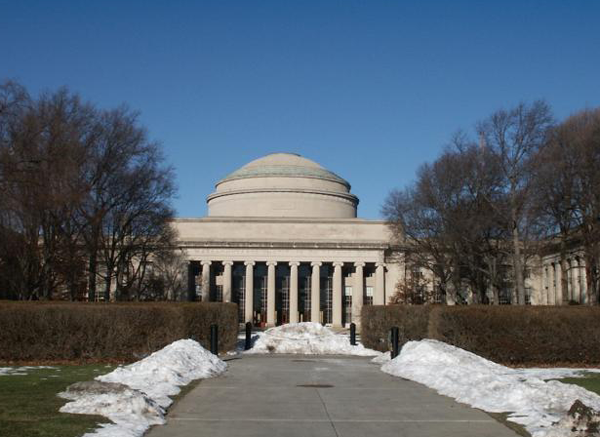
\includegraphics[width=0.9\columnwidth]{Figure1}
%\caption{With Caption Below, be sure to have a good resolution image
%  (see item D within the preparation instructions).}
%\label{fig:figure1}
%\end{figure}


%\begin{table}
%  \centering
%  \begin{tabular}{|c|c|c|}
%    \hline
%    \tabhead{Objects} &
%    \multicolumn{1}{|p{0.3\columnwidth}|}{\centering\tabhead{Caption --- pre-2002}} &
%    \multicolumn{1}{|p{0.4\columnwidth}|}{\centering\tabhead{Caption --- 2003 and afterwards}} \\
%    \hline
%    Tables & Above & Below \\
%    \hline
%    Figures & Below & Below \\
%    \hline
%  \end{tabular}
%  \caption{Table captions should be placed below the table.}
%  \label{tab:table1}
%\end{table}

%It is important that you write for the SIGCHI audience.  Please read
%previous years' Proceedings to understand the writing style and
%conventions that successful authors have used.  It is particularly
%important that you state clearly what you have done, not merely what
%you plan to do, and explain how your work is different from previously
%published work, i.e., what is the unique contribution that your work
%makes to the field?  Please consider what the reader will learn from
%your submission, and how they will find your work useful.  If you
%write with these questions in mind, your work is more likely to be
%successful, both in being accepted into the Conference, and in
%influencing the work of our field.

\section{Acknowledgments}
This research was supported in part by the National Science Foundation under award CCF-0424422 (TRUST). One of the authors (T.M.) acknowledges support by the Swiss National Science Foundation (Grant Nr.  PA00P2-145368).

% Balancing columns in a ref list is a bit of a pain because you
% either use a hack like flushend or balance, or manually insert
% a column break.  http://www.tex.ac.uk/cgi-bin/texfaq2html?label=balance
% multicols doesn't work because we're already in two-column mode,
% and flushend isn't awesome, so I choose balance.  See this
% for more info: http://cs.brown.edu/system/software/latex/doc/balance.pdf
%
% Note that in a perfect world balance wants to be in the first
% column of the last page.
%
% If balance doesn't work for you, you can remove that and
% hard-code a column break into the bbl file right before you
% submit:
%
% http://stackoverflow.com/questions/2149854/how-to-manually-equalize-columns-
% in-an-ieee-paper-if-using-bibtex
%
% Or, just remove \balance and give up on balancing the last page.
%

\balance

% If you want to use smaller typesetting for the reference list,
% uncomment the following line:
% \small

%% to generate the bib
%\bibliographystyle{acm-sigchi}
%\bibliography{../tmaillart.bib}
\input{cscw2015_tight.bbl}
\end{document}
